% The research loop: how both models' settings were searched (revision, November 2026).
% Numbers come from paper/generated/tab_loop.tex and the figures, all built from results/research/*/log.jsonl
% by paper/figs/make_loop_figures.py.
\section{Searching the settings of both models}
\label{sec:loop}

Both models were tuned with the same procedure on every data set. On the windows the searches
scored, tuning improved LightGBM on all \loopImprovedLgb{} data sets and the world model on \loopImprovedWm{}, and the gains
were mostly small next to the differences between data sets. The held-out window agreed with the
search windows only weakly, so the paper judges the models on later windows the searches never
saw. Table~\ref{tab:loop} gives every search from its starting settings to its final settings, and
Figure~\ref{fig:looppath} shows every run in the order it was made.

\subsection{The procedure}

The procedure is a fixed loop, written down before it ran, that changes one setting at a time. It
starts from the settings the first version of this paper used. Each change on a menu fixed in
advance is run once, on one seed, on top of the best settings so far. Every change that beats the
best settings on that seed is run on two more seeds. The best of those is kept if its mean over
three seeds beats the best settings' mean by at least the keep bar, which is the spread of the
three seeds of the starting settings. The loop then starts a new round from the new best and stops
when a round keeps nothing. A change cannot be kept because one seed was lucky, and the bar is set
by the model's own noise on that data set before any change is tried.

The windows the loop scores lie before every window this paper reports. The latest of them is held
out: it is scored for every three-seed run and never used to decide. The menus differ between the
models, because the models have different settings, but each covers what a practitioner would try
first: for the world model the loss weights, the roll-forward, training length, learning rate and
batch, weight averaging and the latent checks of Section~\ref{sec:models}; for LightGBM the
number of leaves, the learning rate and number of rounds, the minimum data in a leaf, the
objective, feature sampling and the lag windows.

After its loop each world model had two more rounds of one change each. The first tried four count
likelihoods that treat weeks with no sales on their own: the negative binomial, the same with a
spread for each item, the zero-inflated negative binomial and the hurdle negative binomial. The
second tried JEPA pretraining of the encoder with the forecast head fitted afterwards at a lower
rate, at two lengths of pretraining. Both used the keep rule above. LightGBM has no counterpart
to either, so it had none. Pretraining used only each data set's own history, so the two models
still saw the same data.

Each model on each data set was searched as a five-copy average, the mean forecast of five fits
with different seeds, except on M5, where both models were single fits. Section~\ref{sec:loopnoise} shows why the
average matters.

\begin{table*}[t]
\centering\footnotesize
\caption{Every search, from starting to final settings. Scores are WRMSSE (lower is better), the mean of three seeds on the search windows and one score on the held-out window, which never decided anything. The keep bar is the seed spread of the starting settings; a change was kept only when its three-seed mean beat the best so far by at least the bar. Tries counts every run, first-seed screens and three-seed confirmations.}
\label{tab:loop}
\begin{tabular}{llrrrrrrp{5.2cm}}
\toprule
Data & Model & Tries & Keep bar & \multicolumn{2}{c}{Starting} & \multicolumn{2}{c}{Final} & Kept, in order \\
& & & & Search & Held-out & Search & Held-out & \\
\midrule
M5 & World model & 59 & 0.013 & 0.570 & 0.550 & 0.533 & 0.534 & feedback, hurdle nb item spread \\
 & LightGBM & 51 & 0.003 & 0.603 & 0.553 & 0.556 & 0.522 & num leaves quarter \\
\addlinespace[2pt]
Favorita & World model & 51 & 0.028 & 0.547 & 0.600 & 0.483 & 0.560 & latent overshooting \\
 & LightGBM & 99 & 0.009 & 0.922 & 0.576 & 0.580 & 0.573 & min data in leaf 4x, objective poisson, learning rate half \\
\addlinespace[2pt]
Frat & World model & 53 & 0.028 & 0.588 & 0.591 & 0.547 & 0.608 & batch half \\
 & LightGBM & 52 & 0.003 & 0.501 & 0.546 & 0.489 & 0.546 & learning rate double \\
\addlinespace[2pt]
Analgesics & World model & 35 & 0.004 & 0.509 & 0.619 & 0.509 & 0.619 & nothing \\
 & LightGBM & 52 & 0.010 & 0.548 & 0.757 & 0.528 & 0.764 & num leaves quarter \\
\addlinespace[2pt]
Bottled juice & World model & 30 & 0.028 & 0.587 & 0.637 & 0.587 & 0.637 & nothing \\
 & LightGBM & 67 & 0.008 & 0.708 & 0.582 & 0.674 & 0.593 & objective poisson, feature fraction 0.8 \\
\addlinespace[2pt]
Cheese & World model & 33 & 0.034 & 0.392 & 0.714 & 0.392 & 0.714 & nothing \\
 & LightGBM & 49 & 0.002 & 0.352 & 0.833 & 0.346 & 0.839 & longer windows \\
\addlinespace[2pt]
Frozen entrees & World model & 95 & 0.007 & 0.246 & 0.251 & 0.216 & 0.241 & total weight 0.1, batch half \\
 & LightGBM & 53 & 0.010 & 0.222 & 0.183 & 0.181 & 0.195 & num leaves 4x \\
\addlinespace[2pt]
Soft drinks & World model & 65 & 0.020 & 0.594 & 0.579 & 0.572 & 0.522 & lr double \\
 & LightGBM & 80 & 0.004 & 0.554 & 0.435 & 0.532 & 0.507 & num leaves quarter, max bin 255 \\
\addlinespace[2pt]
Snacks & World model & 42 & 0.018 & 0.439 & 0.568 & 0.400 & 0.608 & negative binomial item spread, jepa hybrid long \\
 & LightGBM & 54 & 0.006 & 0.358 & 0.425 & 0.351 & 0.424 & rounds double \\
\addlinespace[2pt]
\bottomrule
\end{tabular}
\end{table*}


\begin{figure*}[t]
\centering
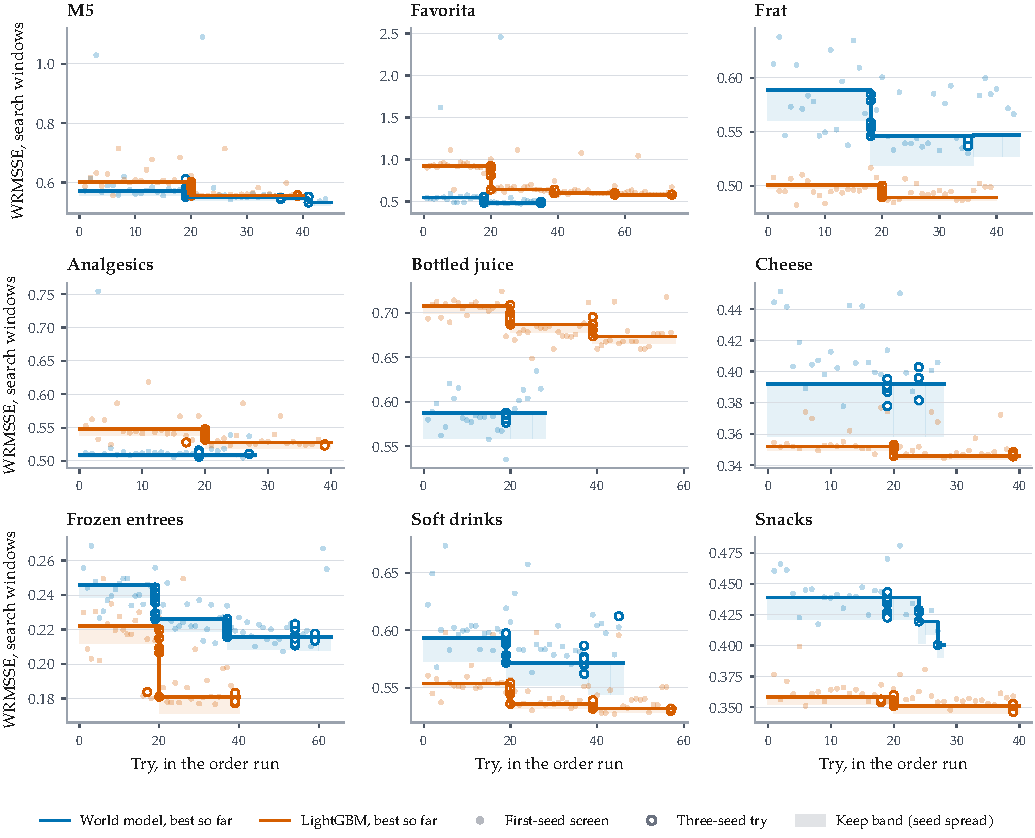
\includegraphics[width=\textwidth]{figs/fig_loop_path.pdf}
\caption{Every run of every search, in the order it was made. Faint dots are first-seed screens,
open circles are three-seed confirmations, and the step line is the best settings so far. The band
under the line is the keep bar: a change had to land below it to be kept. The world model's line
runs on into its likelihood and JEPA rounds after its own loop ends.}
\label{fig:looppath}
\end{figure*}

\subsection{What the searches kept}

The searches made \loopTries{} runs, \loopTriesWm{} of the world model and \loopTriesLgb{} of LightGBM, and kept \loopKept{} changes, \loopKeptWm{} for the world model and \loopKeptLgb{} for LightGBM.
LightGBM kept at least one change on every data set and the world model kept nothing on three of
the six Dominick's categories. No single change helped the world model everywhere
(Figure~\ref{fig:loopheat}). Weighting the loss toward high-volume series made the first seed worse on most data sets. The seven-step latent
check, kept on Favorita, was among the changes that moved Favorita most and did little elsewhere.

On the search windows the world model improved on \loopImprovedWm{} of the nine data sets and LightGBM on all
\loopImprovedLgb{} (Figure~\ref{fig:loopslopes}). The largest gain of either model was LightGBM on \loopGainLgbSet{},
from \loopGainLgbFrom{} to \loopGainLgbTo{}. The world model's largest was on \loopGainWmSet{}, from \loopGainWmFrom{} to \loopGainWmTo{}.

\begin{figure}[t]
\centering
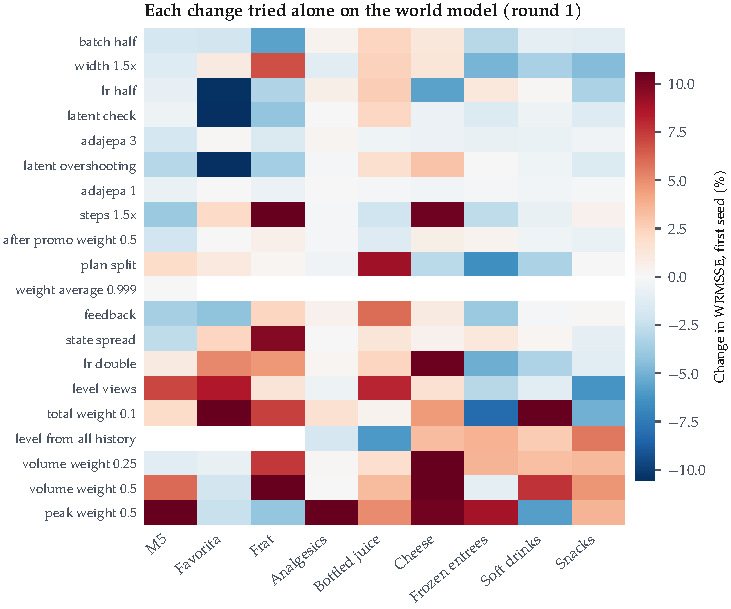
\includegraphics[width=\columnwidth]{figs/fig_loop_heat.pdf}
\caption{Each change tried alone on the world model in the first round, against that data set's
starting settings on the first seed. Blue is better. A blank cell is a change that was not on that
data set's menu.}
\label{fig:loopheat}
\end{figure}

\subsection{Did the held-out window agree?}

Only partly. Across every three-seed run, the change on the search windows and the change on the
held-out window are correlated at \loopHeldCorrWm{} for the world model and \loopHeldCorrLgb{} for LightGBM
(Figure~\ref{fig:loopheldout}). A change that helps on the search windows is a weak guide to the
next window. The world model's final settings were worse than its starting settings on the
held-out window on \loopHeldWorseWm{} data sets, most on \loopHeldWorstWmSet{} (\loopHeldWorstWmFrom{} to \loopHeldWorstWmTo{}), and
LightGBM's on \loopHeldWorseLgb{}, most on \loopHeldWorstLgbSet{} (\loopHeldWorstLgbFrom{} to \loopHeldWorstLgbTo{}). This is why the paper reports the final settings on windows that the
searches never saw, in Section~\ref{sec:results}, and not the search scores.

\begin{figure}[t]
\centering
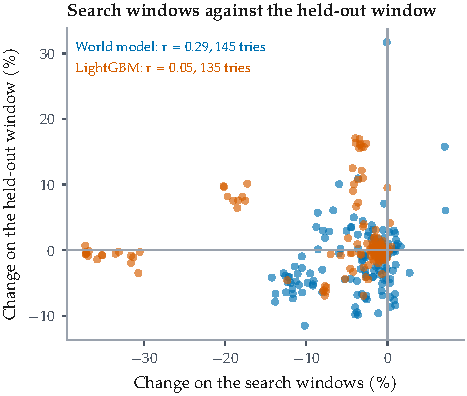
\includegraphics[width=\columnwidth]{figs/fig_loop_heldout.pdf}
\caption{Each three-seed run's change on the search windows against its change on the held-out
window, both against the starting settings of its search.}
\label{fig:loopheldout}
\end{figure}

\subsection{Seed noise, one copy against five}
\label{sec:loopnoise}

A single world-model fit is noisy enough to hide most of the changes the loop tries. On the six
Dominick's categories the three seeds of the starting settings differ from their mean by a
standard deviation of \loopSeedSdOne\% for a single fit and \loopSeedSdFive\% for a five-copy average
(Figure~\ref{fig:loopnoise}). The
single-fit search on cheese had a bar of \loopOneCheBar{} and kept nothing; with the average the bars on the
Dominick's categories were between \loopBarLoWm{} and \loopBarHiWm{}. LightGBM's seeds differ much less, and its
bars were between \loopBarLoLgb{} and \loopBarHiLgb{}.

\begin{figure}[t]
\centering
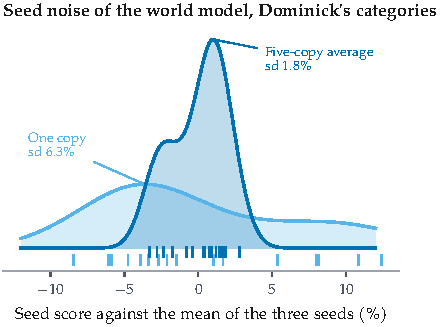
\includegraphics[width=\columnwidth]{figs/fig_loop_noise.pdf}
\caption{The starting settings' three seed scores on each Dominick's category, as a share of their
mean, for a single world-model fit and for the five-copy average. Ticks are the scores.}
\label{fig:loopnoise}
\end{figure}

\begin{figure*}[t]
\centering
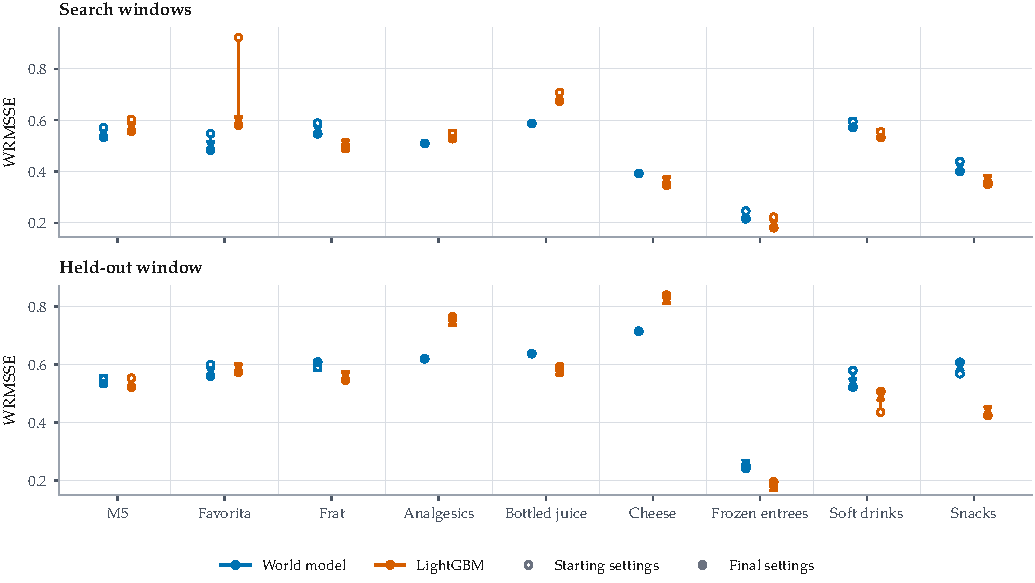
\includegraphics[width=\textwidth]{figs/fig_loop_slopes.pdf}
\caption{Each model's starting and final settings on each data set. Open circles are the starting
settings and filled circles the final settings, on the search windows (top) and the held-out
window (bottom).}
\label{fig:loopslopes}
\end{figure*}
